%!TEX root = ../these.tex

\subsection*{%
Решение задач большой размерности
}
\label{sec:pcgtsp.ufa}

Предлагаемый алгоритм существенно увеличивает размеры
экземпляров задач PCGTSP,
для которых может быть получено точное решение с
$\approx 30$ кластеров
\cite{bi:RoMa}
до 50--60,
а в некоторых случаях до
$\approx 150$
(в зависимости от вложенности).
Вместе с тем,
задачи большой размерности
(сотни и тысячи кластеров)
все еще остаются недоступными для точного
решения
(за разумное время),
однако для них легко находятся
практически приемлемые решения.

Примеры таких маршрутов приведены на
рис.~\ref{fig:pcgtsp.ufa}.
Раскройные планы предоставлены
М.А.~Верхотуровым,
численные данные приведены
в~табл.~\ref{tab:pcgtsp.ufa}.

Для каждого раскройного плана
строилось 4 разных экземпляра задачи
PCGTSP
за счёт дискретизации контуров деталей с разным
шагом ---
от 25~мм до 1000~мм
(в последнем случае фактически получалась
задача TSP).
Решения на рис.~\ref{fig:pcgtsp.ufa}.
получены при дискретизации с шагом
50~мм.
Для каждого экземпляра приведены
количество получившихся узлов,
нижняя оценка,
полученная описанный в данной главе алгоритмом,
длина решения, полученного эвристикой PCGLNS
и оценка его погрешности.
Также приведены длины решения
исходной непрерывной задачи CCP
алгоритмом,
описанным в главе~\ref{ch:ccp}
(см. Табл.~\ref{tab:ccp.ufa}
на стр.~\pageref{tab:ccp.ufa})
и на сколько решение дискретной задачи
превышает решение соответствующей
непрерывной задачи.

\begin{figure}
  \centering
  \subfloat[$m=424$ кластера]{
    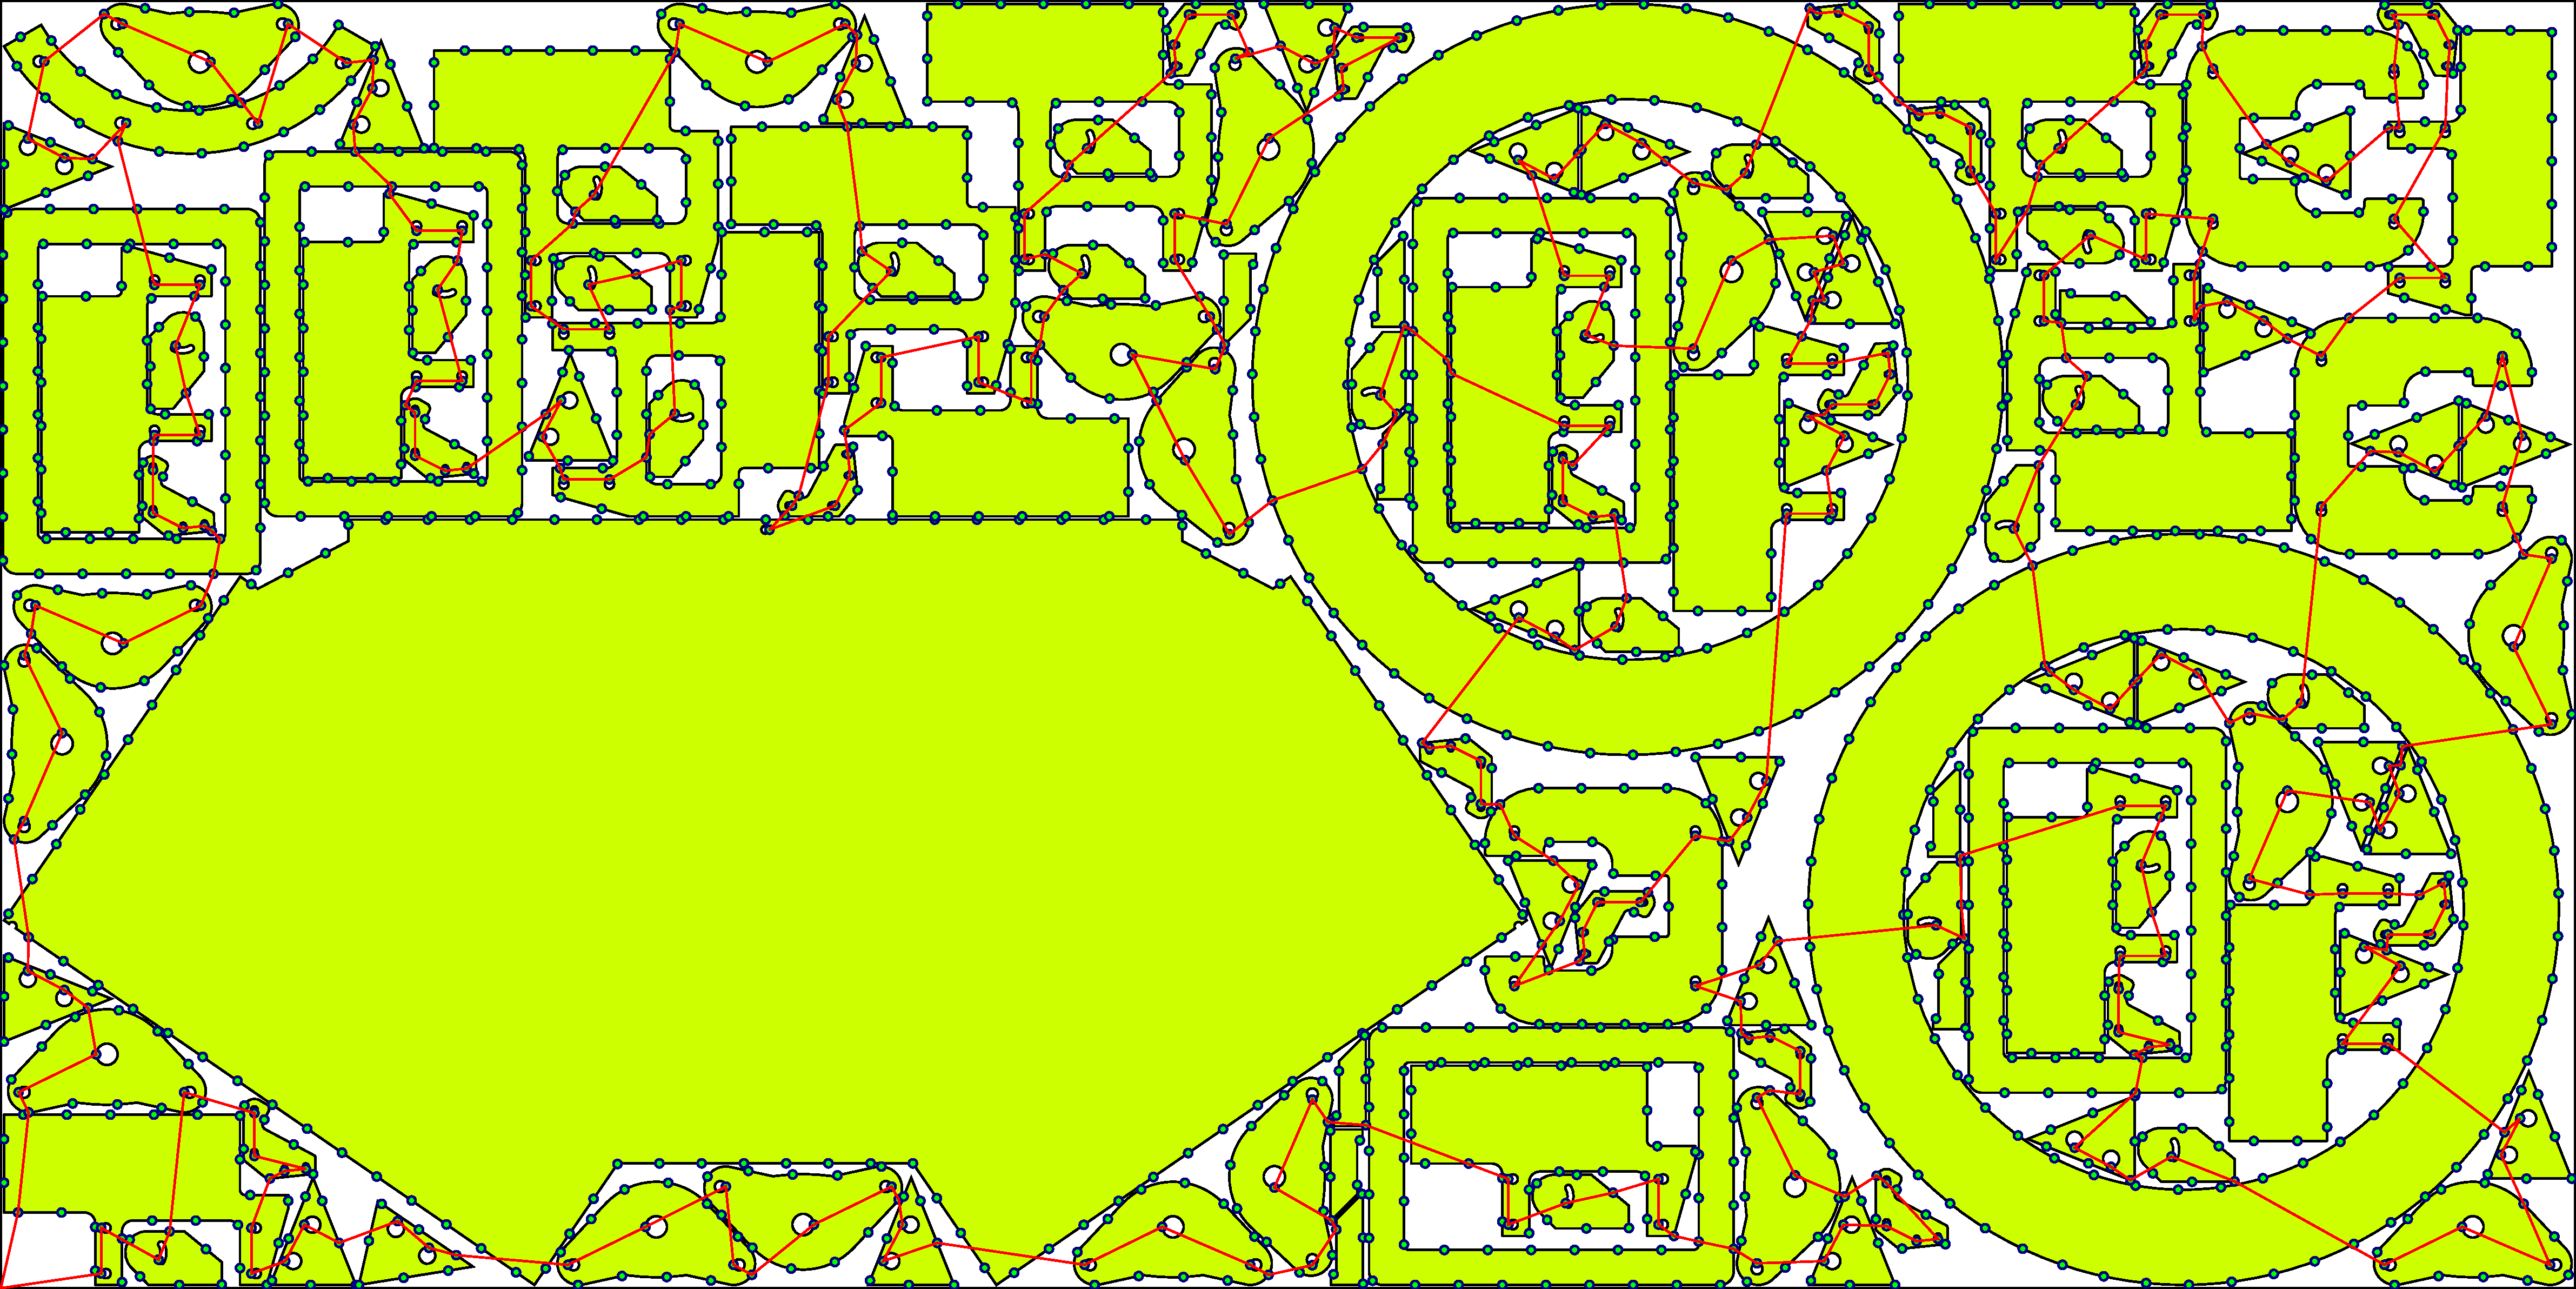
\includegraphics[width=0.95\textwidth]{ufa/a.pcglns.pdf}
  }
  \\
  \subfloat[$m=621$ кластер]{
    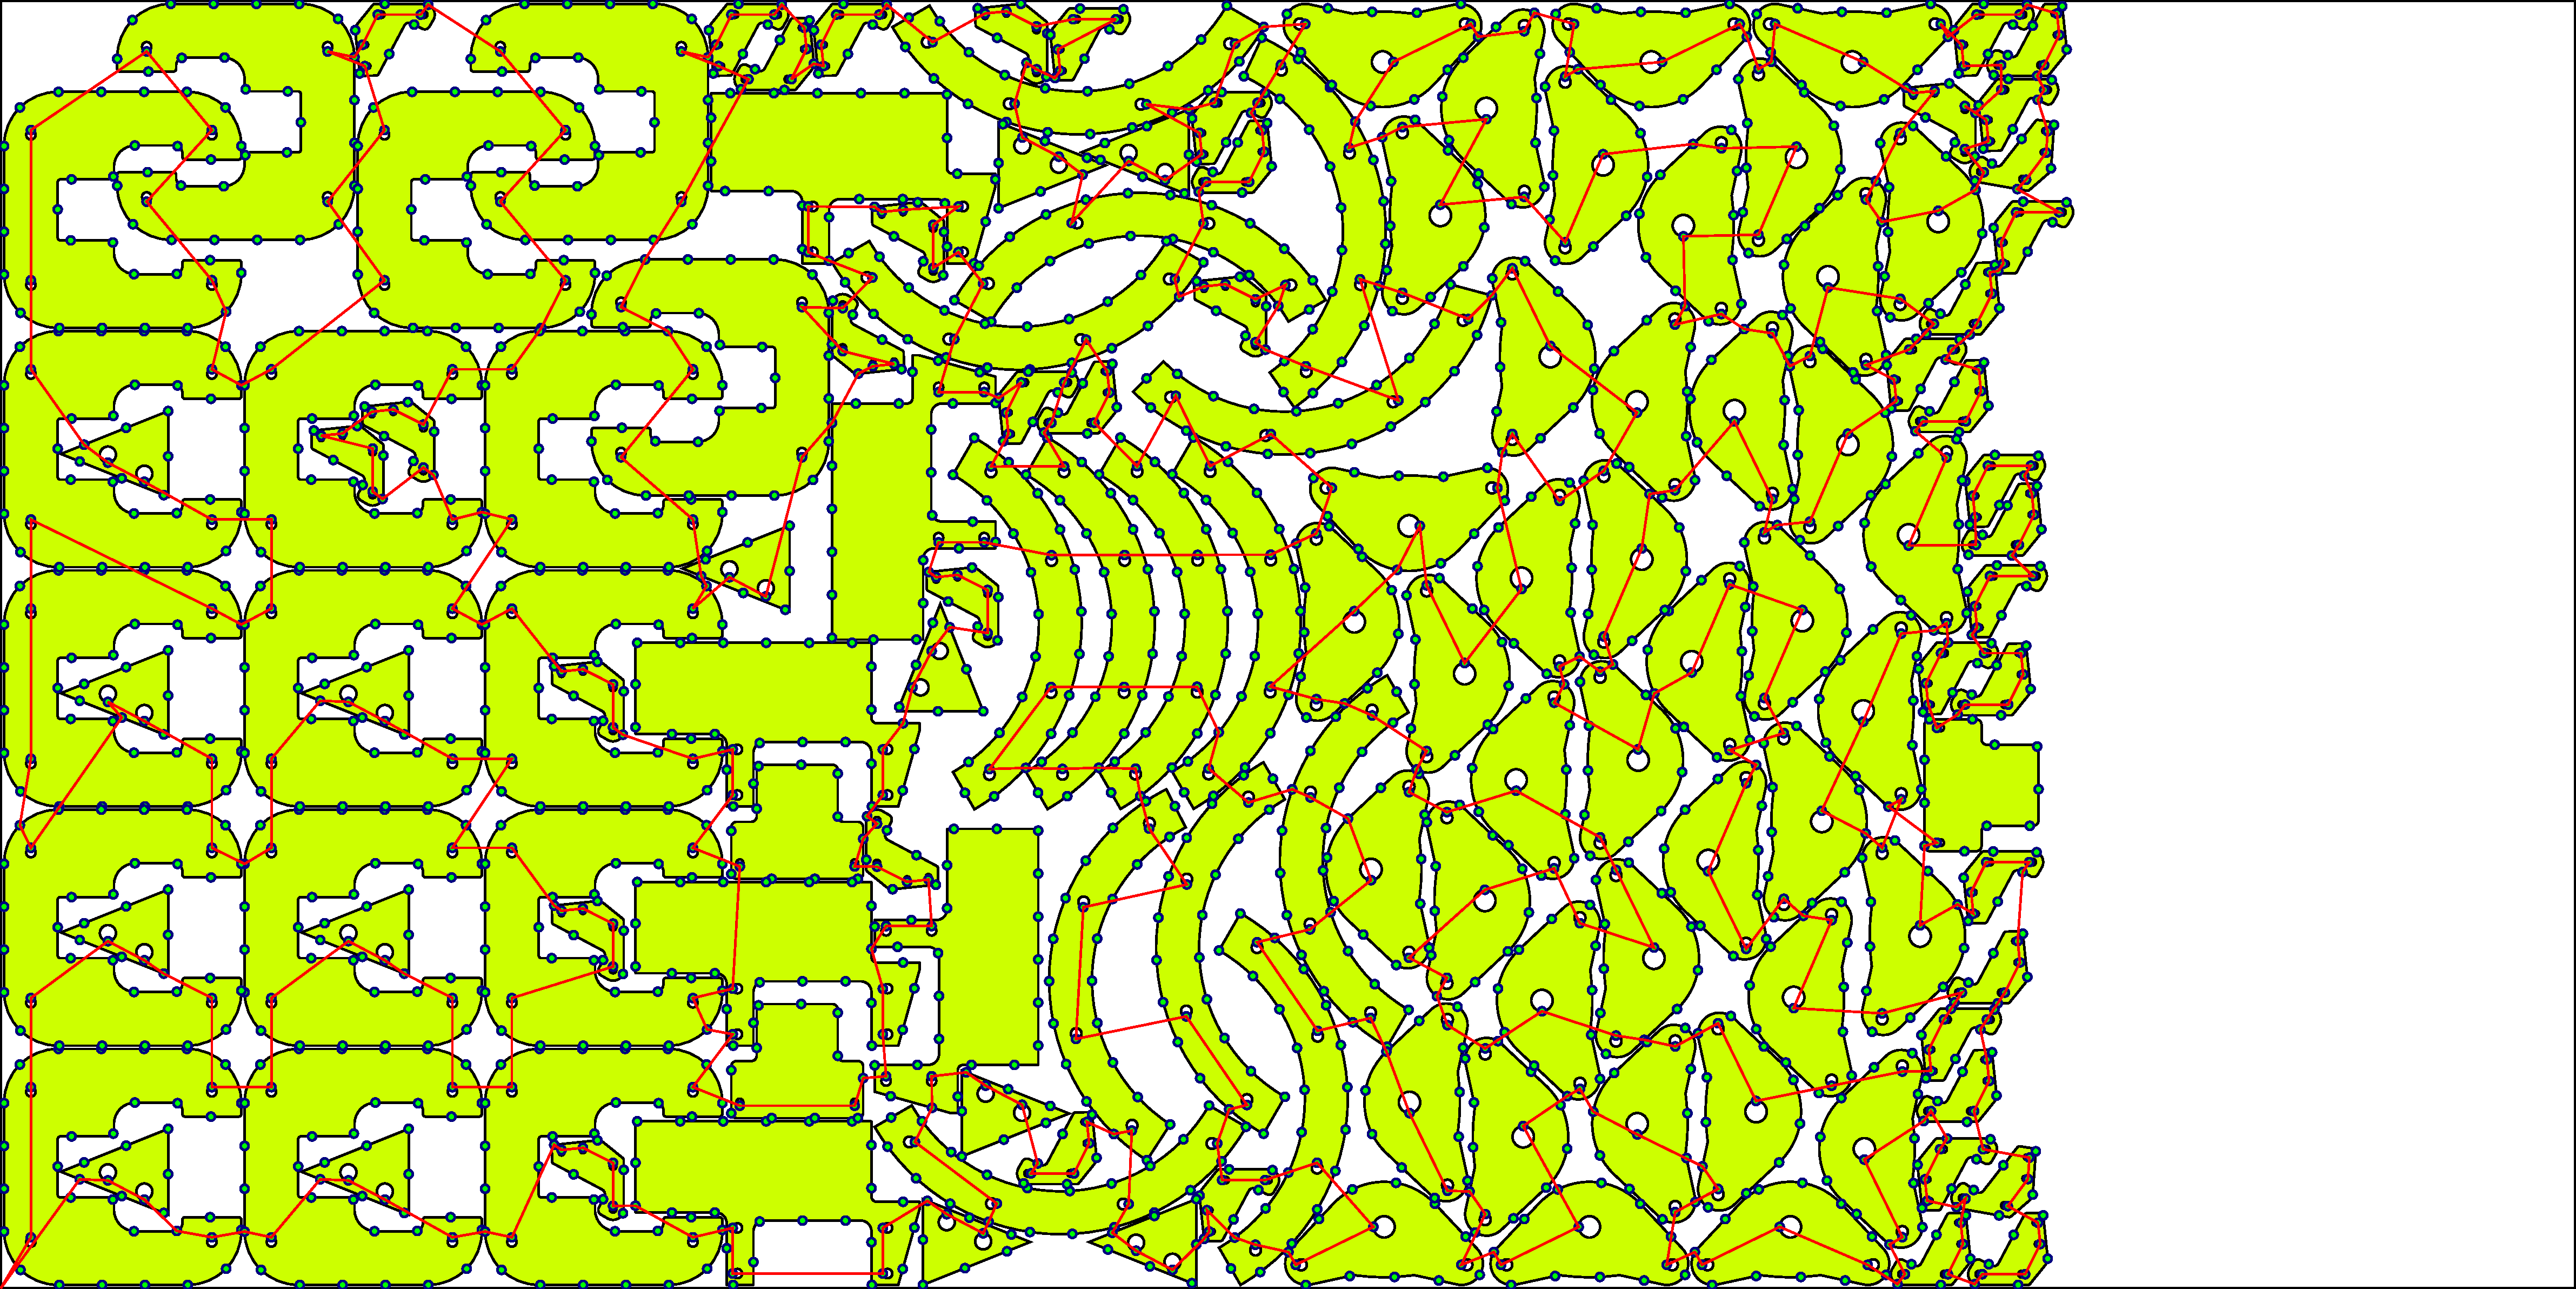
\includegraphics[width=0.95\textwidth]{ufa/b.pcglns.pdf}
  }
  \caption{Решения задач PCGTSP большой размерности}
  \label{fig:pcgtsp.ufa}
\end{figure}

\begin{table}
  \centering
  \caption{Результаты решения задач PCGTSP большой размерности}
  \label{tab:pcgtsp.ufa}
  \small
  \begin{tabular}{|r|rrrr|rrrr|}
  \hline
  Кластеров &
    \multicolumn{4}{c|}{424} &
    \multicolumn{4}{c|}{621} \\ \hline
  Шаг, мм &
    {25} &
    {50} &
    {100} &
    1000 &
    {25} &
    {50} &
    {100} &
    1000 \\ \hline
  Узлов &
    {4023} &
    {2062} &
    {1134} &
    431 &
    {4190} &
    {2253} &
    {1320} &
    621 \\ \hline
  LB, мм &
    {15818} &
    {17457} &
    {18561} &
    25436 &
    {26132} &
    {27663} &
    {28349} &
    34487 \\ \hline
  PCGLNS, мм &
    {23374} &
    {24490} &
    {25421} &
    34315 &
    {33522} &
    {34691} &
    {35410} &
    45870 \\ \hline
  gap, \% &
    {47,77\%} &
    {40,29\%} &
    {36,96\%} &
    34,91\% &
    {28,28\%} &
    {25,41\%} &
    {24,91\%} &
    33,01\% \\ \hline
  CCP, мм &
    \multicolumn{4}{c|}{22609} &
    \multicolumn{4}{c|}{32051} \\ \hline
  GTSP / CCP &
    {3,38\%} &
    {8,32\%} &
    {12,44\%} &
    51,78\% &
    {4,59\%} &
    {8,24\%} &
    {10,48\%} &
    43,12\% \\ \hline
  \end{tabular}
\end{table}
